\documentclass[a4paper]{article}
\usepackage[english]{babel}
\usepackage{multicol}
\usepackage{amsmath}
\usepackage{amsfonts}
\usepackage{amssymb}
\usepackage[font=scriptsize]{caption}
\usepackage{parskip}
\usepackage[a4paper, margin=1in, total={6in, 8in}]{geometry}
\usepackage{titling}
\usepackage{subcaption}
\usepackage{float}
\usepackage{placeins}
\usepackage{graphicx}
\usepackage[backend=biber,style=numeric]{biblatex}
\addbibresource{references.bib}

\parskip = 6pt plus 2pt minus 2pt
\setlength{\droptitle}{-2cm}

\title{HW9 - Computer Simulation II}
\author{Schewtschik, Guilherme (3748052)}
\date{\today}

\begin{document}
\maketitle

\section{}

Using the histogram rewightint method we get

\begin{figure}[ht]
    \centering
    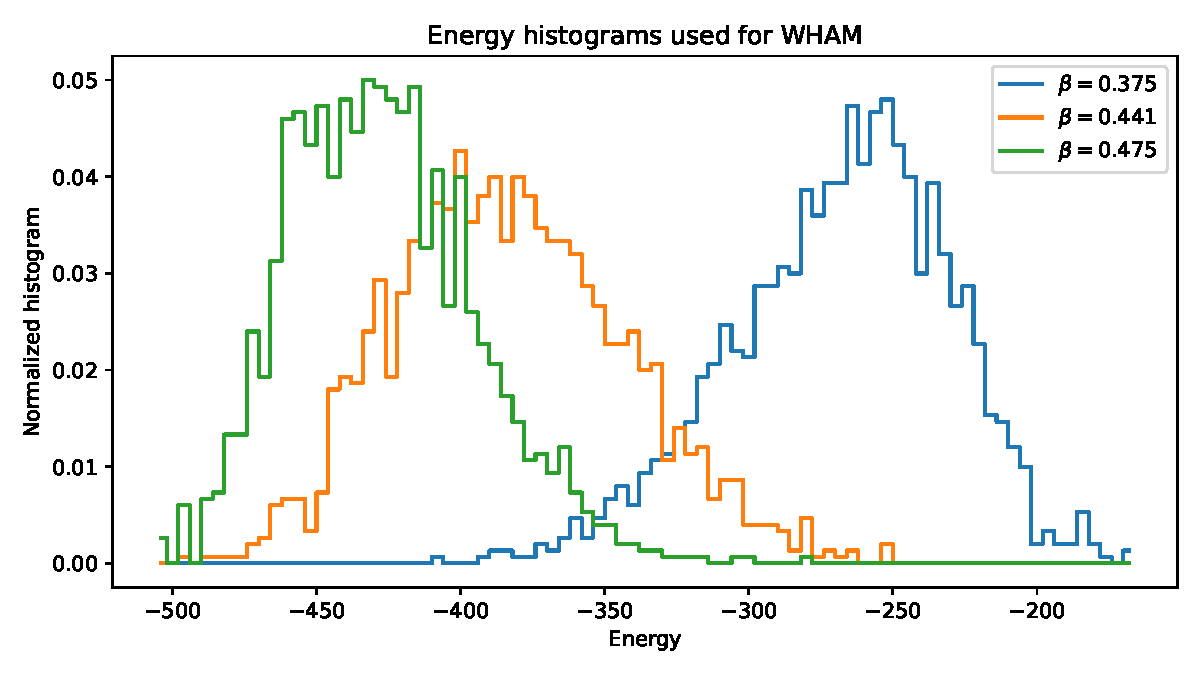
\includegraphics[width=0.5\linewidth]{figures/hw9_problem17_histograms.pdf}
    \caption{Energy histograms.}
    \label{fig:wham_hist}
\end{figure}

\begin{figure}[ht]
    \centering
    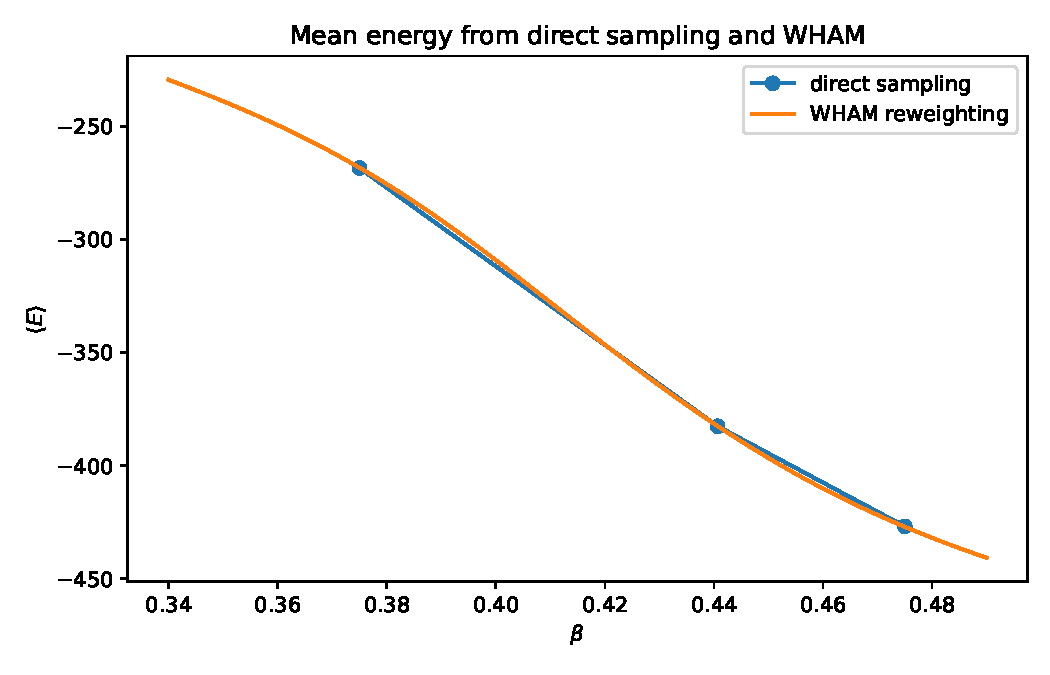
\includegraphics[width=0.5\linewidth]{figures/hw9_problem17_energy_vs_beta.pdf}
    \caption{Mean energy from direct sampling and from WHAM.}
    \label{fig:wham_energy}
\end{figure}

The WHAM estimate agrees well with the direct measurements near the simulated values and provides a smooth interpolation of the energy curve between the three simulation points.

\newpage

\section{}

Using the improve estimator for the susceptability we get:

\begin{figure}[ht]
    \centering
    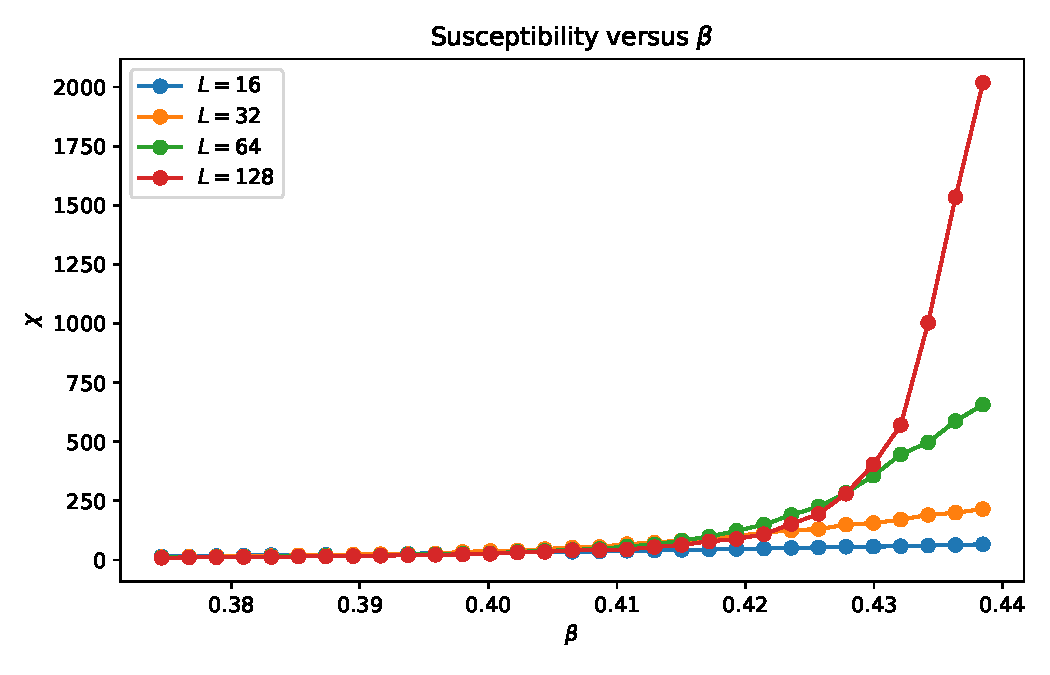
\includegraphics[width=0.5\linewidth]{figures/hw9_problem18_chi_vs_beta.pdf}
    \caption{Susceptibility as a function of $\beta$ for several lattice sizes.}
    \label{fig:chi_beta}
\end{figure}

\begin{figure}[ht]
    \centering
    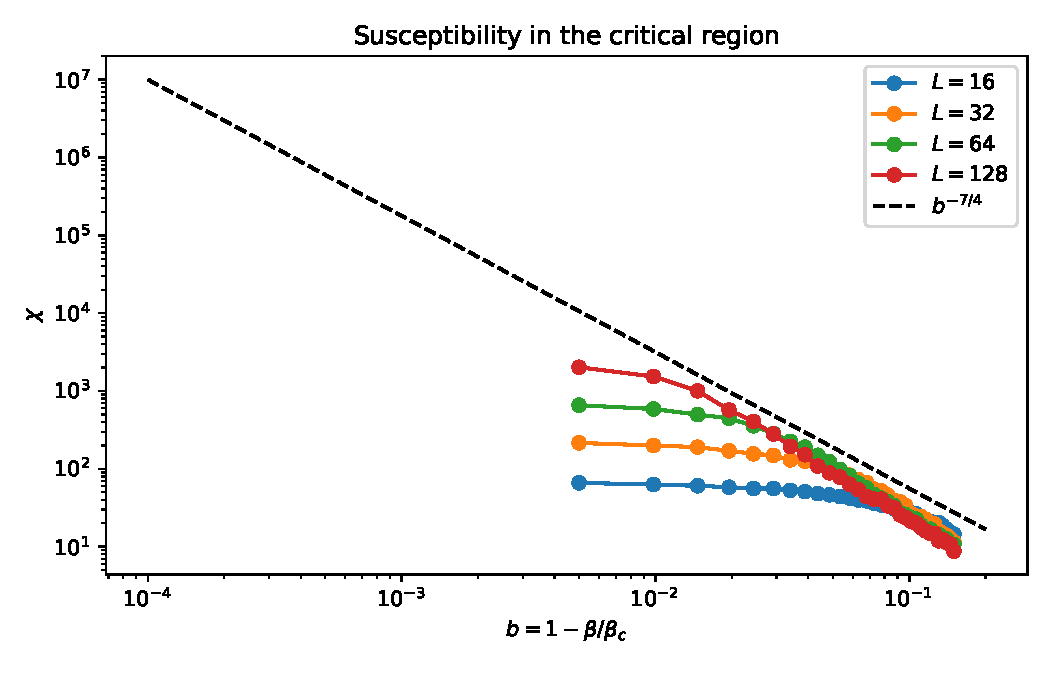
\includegraphics[width=0.5\linewidth]{figures/hw9_problem18_loglog_vs_b.pdf}
    \caption{Log-log plot of $\chi$ versus $b=1-\beta/\beta_c$ with the expected power law $b^{-7/4}$.}
    \label{fig:chi_b}
\end{figure}

\begin{figure}[ht]
    \centering
    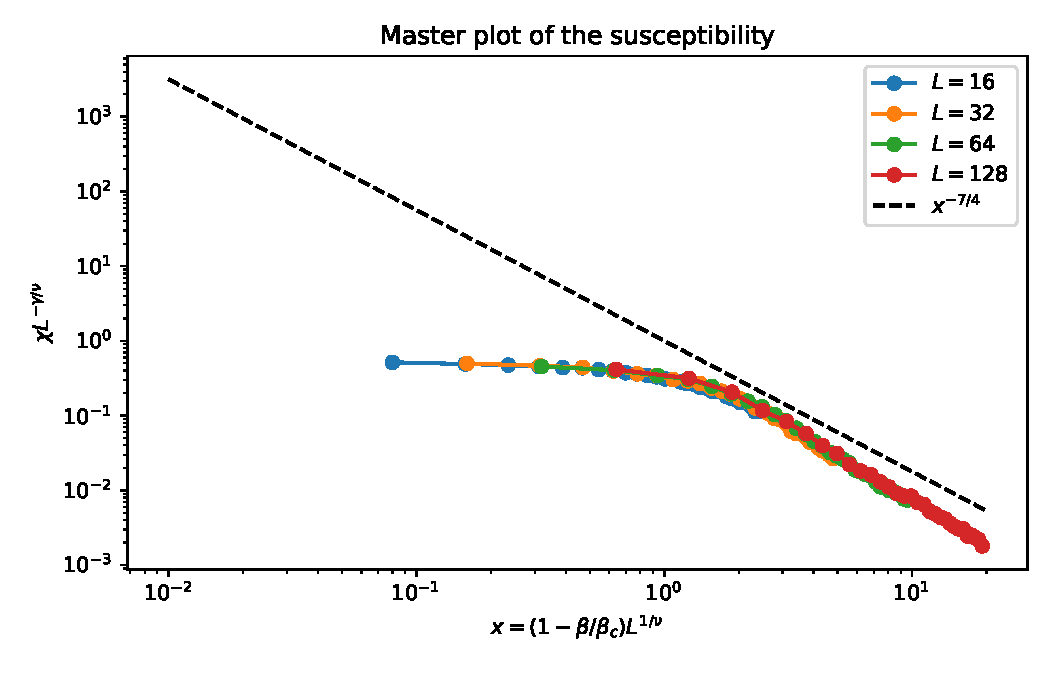
\includegraphics[width=0.5\linewidth]{figures/hw9_problem18_master_plot.pdf}
    \caption{Master plot of $\chi L^{-\gamma/\nu}$ versus $x=(1-\beta/\beta_c)L^{1/\nu}$, using $\nu=1$ and $\gamma=7/4$.}
    \label{fig:chi_master}
\end{figure}

The susceptibility grows strongly near the critical point $\beta = 0.44$ for $L > 16$, scalling with lattice size.
In the second plot we can see that the susceptability approaches the expected near $\beta_c$ but still shows big dependence on
lattice size, while the master plot shows a lattice size independent result.
\printbibliography

\end{document}